\documentclass{beamer}


% Paquetes
\usepackage[T1]{fontenc}    % Para escribir en español
\usepackage{hyperref}    % Para hacer links a la web
\usepackage{listings}    % Para incluir código
\usepackage{graphicx}    % Para incluir imágenes

% Setup imagenes
\graphicspath{ {out/}}


% Estilos
\usetheme{Luebeck}


% Info para la title page
\title{Concurrencia a Museos de Argentina}
\subtitle{Relación con otros consumos culturales}
\author{Nazareno Magallanes \and Javier Spina \and Lautaro Terreno}
\institute[ECyT]
{
  Escuela de Ciencia y Tecnología
  \and
  Universidad Nacional de San Martín
}
\date{Noviembre 2022}


% Inicio del documento
\begin{document}

\frame{\titlepage}

% Presentación
\begin{frame}
\frametitle{Presentación del \textit{dataset}}

\begin{columns}
\column{0.45\textwidth}
\begin{figure}
\centering
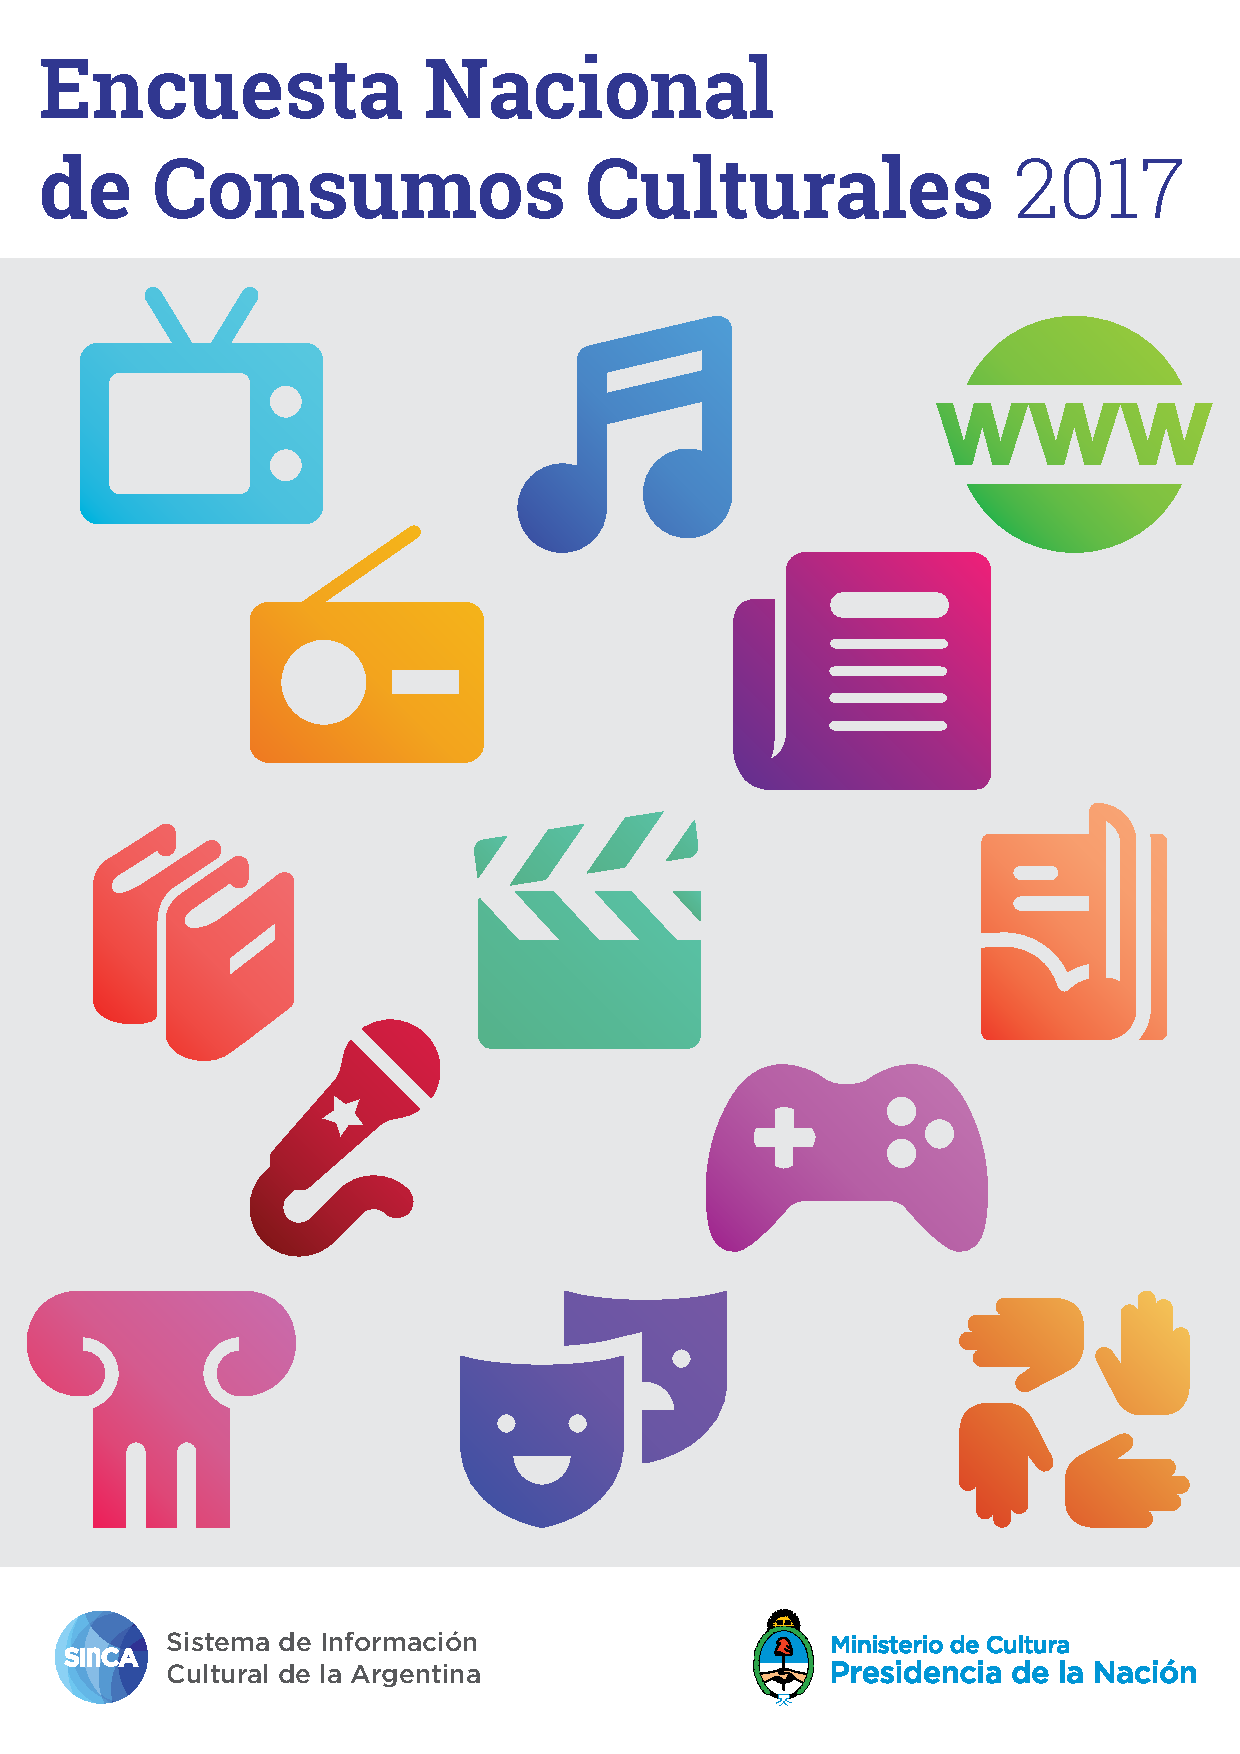
\includegraphics[height=0.7\textheight]{encc_informe_portada.pdf}
\label{fig:portada_encc}
\end{figure}

\column{0.45\textwidth}
\begin{itemize}
\item<1->Se trabajó con el \textit{dataset} asociado a la \textbf{Encuesta Nacional de Consumos Culturales} realizada en 2017. 
\item<2->Se complementó con los datos abiertos de los Museos de Argentina.
\item<3->Fuente: Ministerio de Cultura de la Nación, disponible en \href{https://datos.cultura.gob.ar/dataset/encuesta-nacional-de-consumos-culturales-2017}{su página web.}
\end{itemize}
\end{columns}

\end{frame}

% Pregunta y contexto
\begin{frame}
\frametitle{La pregunta y su contexto}

\begin{block}{La pregunta}
¿Cómo aumentar la concurrencia a los museos?
\end{block}

\begin{figure}
\centering
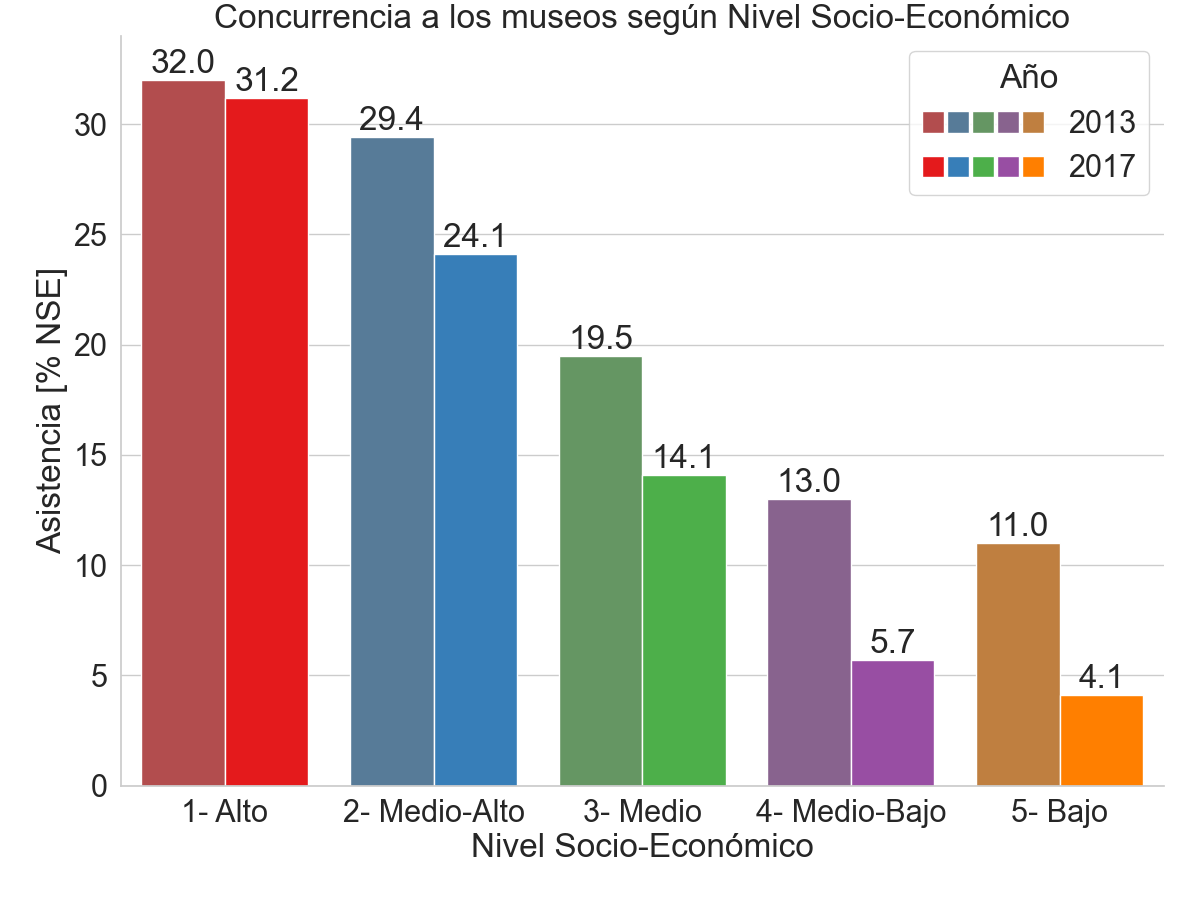
\includegraphics[height=0.6\textheight]{asist_museo_nse_x100}
\label{fig:asist_museo_nse}
\end{figure}

\end{frame}

% Cantidad de museos y entradas
\begin{frame}
\frametitle{Entradas expedidas en cada región}

\begin{figure}
\centering
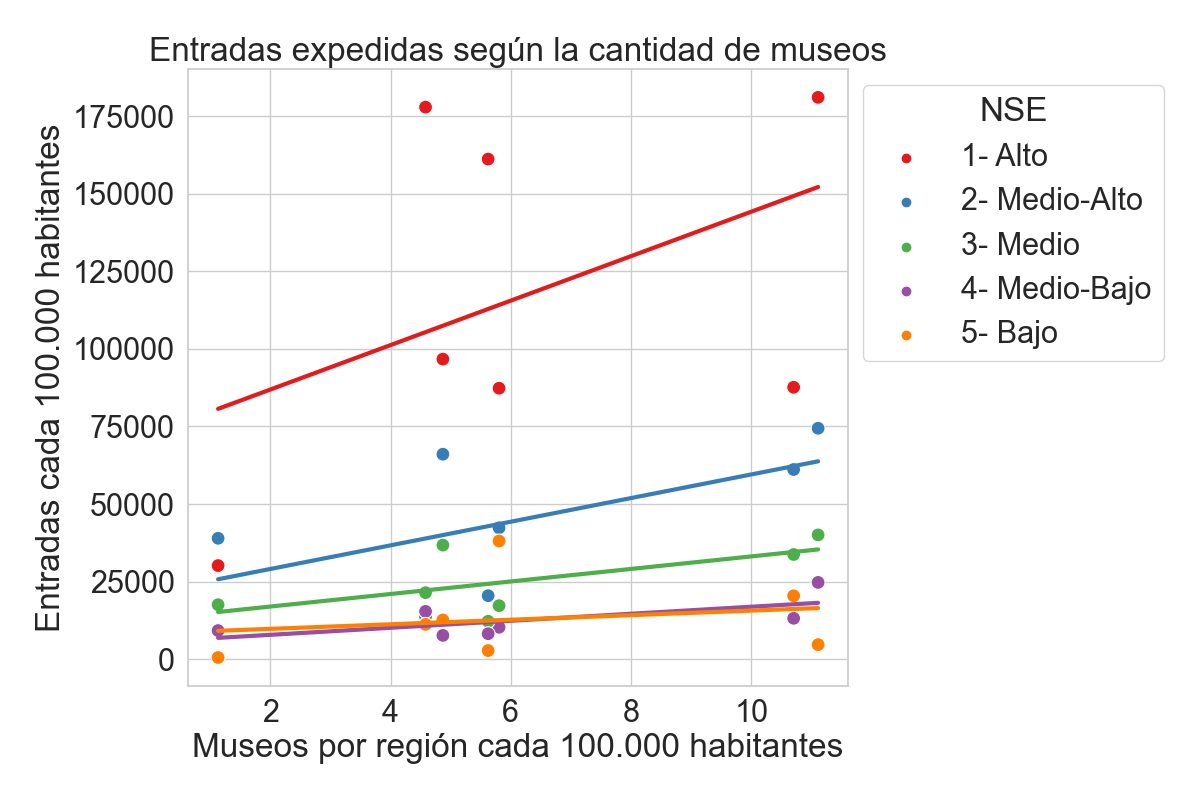
\includegraphics[width=\textwidth]{modelo_entrada_museo}
\label{fig:modelo_entrada_museo}
\end{figure}

\end{frame}

\end{document}
